\documentclass[../main.tex]{subfiles}
\graphicspath{{../images/}}

\begin{document}
\subsection*{Lecture 12: \hfill  2/16/24}
\hrule \vspace{10px}
\section{Lagrange's Equations}

From last time: we defined the path
\begin{align*}
    S = \int_a^b f(x, y(x), y'(x)) \dd x
\end{align*}
Goal: find $y(x)$ that minimizes $S$ using EL
\begin{align*}
    \text{EL:} \quad \pdv{f}{y} - \dv{x}(\pdv{f}{y'}) = 0
\end{align*}
where near the minimum $\delta S = 0$. From the EL, $y(x)$ is a stationary point of $S$(could also
be a maximum!). 

\paragraph*{Lagrangian} In Classical Mechanics, we use a specific form 
\begin{align*}
    \mathcal{L} = T - V
\end{align*}
this has the units of energy and the action $S$ has the units $[S] = [E \cdot T]$ similar to
planck's constant $\hbar$.
\paragraph*{3D Cartesian} $x, y, z = q_1, q_2, q_3$
\begin{align*}
    T &= \frac{1}{2} m v^2 = \frac{1}{2} m (\dot x^2 + \dot y^2 + \dot z^2) \\
    U &= U(x, y, z)
\end{align*}
where the potential energy only depends on the position and $T$ only depends on the velocity, so 
\begin{align*} 
    \mathcal{L} = \frac{1}{2} m (\dot x^2 + \dot y^2 + \dot z^2) - U(x, y, z)
\end{align*}
and the EL equation for the Lagrangian is
\begin{align*}
    \pdv{\mathcal{L}}{q_i} = \dv{t} \pdv{\mathcal{L}}{\dot q_i}
\end{align*}
For the 3D case, we have 3 equations of motion: For $x$ we have 
\begin{align*}
    \pdv{\mathcal{L}}{x} = - \pdv{U}{x}, \quad \pdv{\mathcal{L}}{\dot x} = m \dot x
\end{align*}
and using the EL equation, we get
\begin{align*}
    -\pdv{U}{x} = \dv{t}(m \dot x) = m \ddot x
\end{align*}
which is Newton's second law $F_x = m a_x$ where $\vb{F} = - \grad U$. We can now get the general form
\begin{align*}
    \vb F = m \vb a
\end{align*}
\paragraph*{Polar Coordinates} $q: (r, \phi)$ we know that
\begin{align*}
    \vb v = v_r \vu r + v_\phi \vu* \phi = \dot r \vu r + r \dot \phi \vu* \phi
\end{align*}
and
\begin{align*}
    U = U(r, \phi), \qquad T = \frac{1}{2} m v^2 = \frac{1}{2} m (\dot r^2 + r^2 \dot \phi^2)
\end{align*}
first we find the parts EL equation for $r$
\begin{align*}
    \pdv{\lagr}{r} &= mr \dot \phi^2 - \pdv{U}{r} \\
    \pdv{\lagr}{\dot r} &= m \dot r
\end{align*}
and the EL equation is
\begin{align*}
    mr \dot \phi^2 - \pdv{U}{r} = \dv{t}(m \dot r) \\
    m(\ddot r - r \dot \phi^2) = - \pdv{U}{r}
\end{align*}
which gives us N2L for $r$. For $\phi$ we have
\begin{align*}
    \pdv{\lagr}{\phi} &= -\pdv{U}{\phi} \\
    \pdv{\lagr}{\dot \phi} &= m r^2 \dot \phi
\end{align*}
and from the EL equation we get
\begin{align*}
    -\pdv{U}{\phi} = \dv{t}(mr^2 \dot \phi ) = m(2 r \dot r \dot \phi + r^2 \ddot \phi)
\end{align*}
dividing both sides by $r$
\begin{align*}
    -\frac{1}{r} \pdv{U}{\phi} = m(r \ddot \phi + 2 \dot r \dot \phi) = -(\grad U)_\phi
\end{align*}
from both forms we know that the two parts of the EL represent the momentum and force:
\begin{align*}
    \pdv{\lagr}{\dot q_i} &= p_i \qqtext{generalized momentum} \\
    \pdv{\lagr}{q_i} &= F_i \qqtext{generalized force} 
\end{align*}
where $F_i = \dv{t} p_i$ is the generalized N2L.
\paragraph*{Example:}  Mass $m$ sliding down a frictionless \emph{moving} ramp $M$. First we choose the
coordinates $x$ moving along withe the ramp and $y$ down in the perpendicular direction. For the
ramp $M$:
\begin{align*}
    T_M = \frac{1}{2} M \dot q_2^2, \quad U_M = 0
\end{align*}
and for the mass $m$: First we decompose the velocity of $m$ into the $x$ and $y$ components
\begin{align*}
    \vb v_m = \dot x \vu x + \dot y \vu y = \vu y(\dot q_1 \sin \alpha)
        + \vu x(\dot q_1 \cos \alpha + \dot q_2)
\end{align*}
and the kinetic and potential energies are
\begin{align*}
    T_m = \frac{1}{2} m v_m^2 = \frac{1}{2} m (\dot q_1^2 + 2 \dot q_1 \dot q_2 \cos \alpha + \dot q_2^2) \\
    U_m = mgy = -mg (\dot q_1 \sin \alpha)
\end{align*}
using the Lagrangian $\mathcal{L} = T - U = T_M + T_m - U_M - U_m$ we get
\begin{align*}
    \pdv{\lagr}{q_2} &= 0, \quad \pdv{\lagr}{\dot q_2} = M \dot q_2 + m \dot q_2 + m \dot q_1 \cos \alpha
\end{align*}
and the EL equation gives us
\begin{align*}
    (M + m) \ddot q_2 + m \ddot q_1 \cos \alpha = 0 \\
    a_2 = \ddot q_2 = -\frac{m \ddot q_1 \cos \alpha}{M + m}
\end{align*}
and for $q_1$ we have
\begin{align*}
    \pdv{\lagr}{q_1} &= mg \sin \alpha,
        \quad \pdv{\lagr}{\dot q_1} = m (\dot q_1 + \dot q_2 \cos \alpha)
\end{align*}
and the EL equation gives us
\begin{align*}
    mg \sin \alpha = m (\ddot q_1 + \ddot q_2 \cos \alpha)
\end{align*}
and since we have two equations and two unknowns, we can solve for $\ddot q_1$ and $\ddot q_2$.
\begin{align*}
    \ddot q_1 = \frac{g \sin \alpha}{1 - \frac{m\cos^2 \alpha}{m + M}} = const \\
    \ddot q_2 = -\frac{m \ddot q_1 \cos \alpha}{M + m} = const
\end{align*}
for $\alpha = 90^\circ$, we get $\ddot q_1 = g$ and $\ddot q_2 = 0$ which is the same as a free falling.
For and infinitely heavy ramp $M \to \infty$, we get $\ddot q_1 = g \sin\alpha$. For $M \to 0$ we
get $\ddot q_1 = g / \sin\alpha$ which doesn't make sense because the force on the mass would be
infinite. The normal force $N \to 0$ as $M \to 0$ and the mass would be in free fall.

\newpage
\subsection*{Lecture 13: \hfill 2/19/24}
\hrule \vspace{10px}

\paragraph*{Review} Lagrangian: For a general integral
\begin{align*}
    S \int f(x,y, y') \dd x
\end{align*}
find $y(x)$ minimizing $S$ using the EL equation
\begin{align*}
    \pdv{f}{y} = \dv{x}(\pdv{f}{y'})
\end{align*}
For Classical Mechanics, we use the Lagrangian in the generalized coordinate system $q_i$ we define
the action $S$ as
\begin{align*}
    S = \int \lagr (q_i, \dot q_i, t) \dd t \qqtext{find} q(t)
\end{align*}
and from the EL equation we get
\begin{align*}
    \pdv{\lagr}{q_i} = \dv{t} \pdv{\lagr}{\dot q_i}
\end{align*}
for each degree of freedom. We define the Lagrangian in CM as the quantity $\lagr = T - U$

\paragraph*{Examples, Examples, and more Examples:} A pendulum but its spining on its axis. We 
first find  the energies:
\begin{figure}[ht]
    \centering
    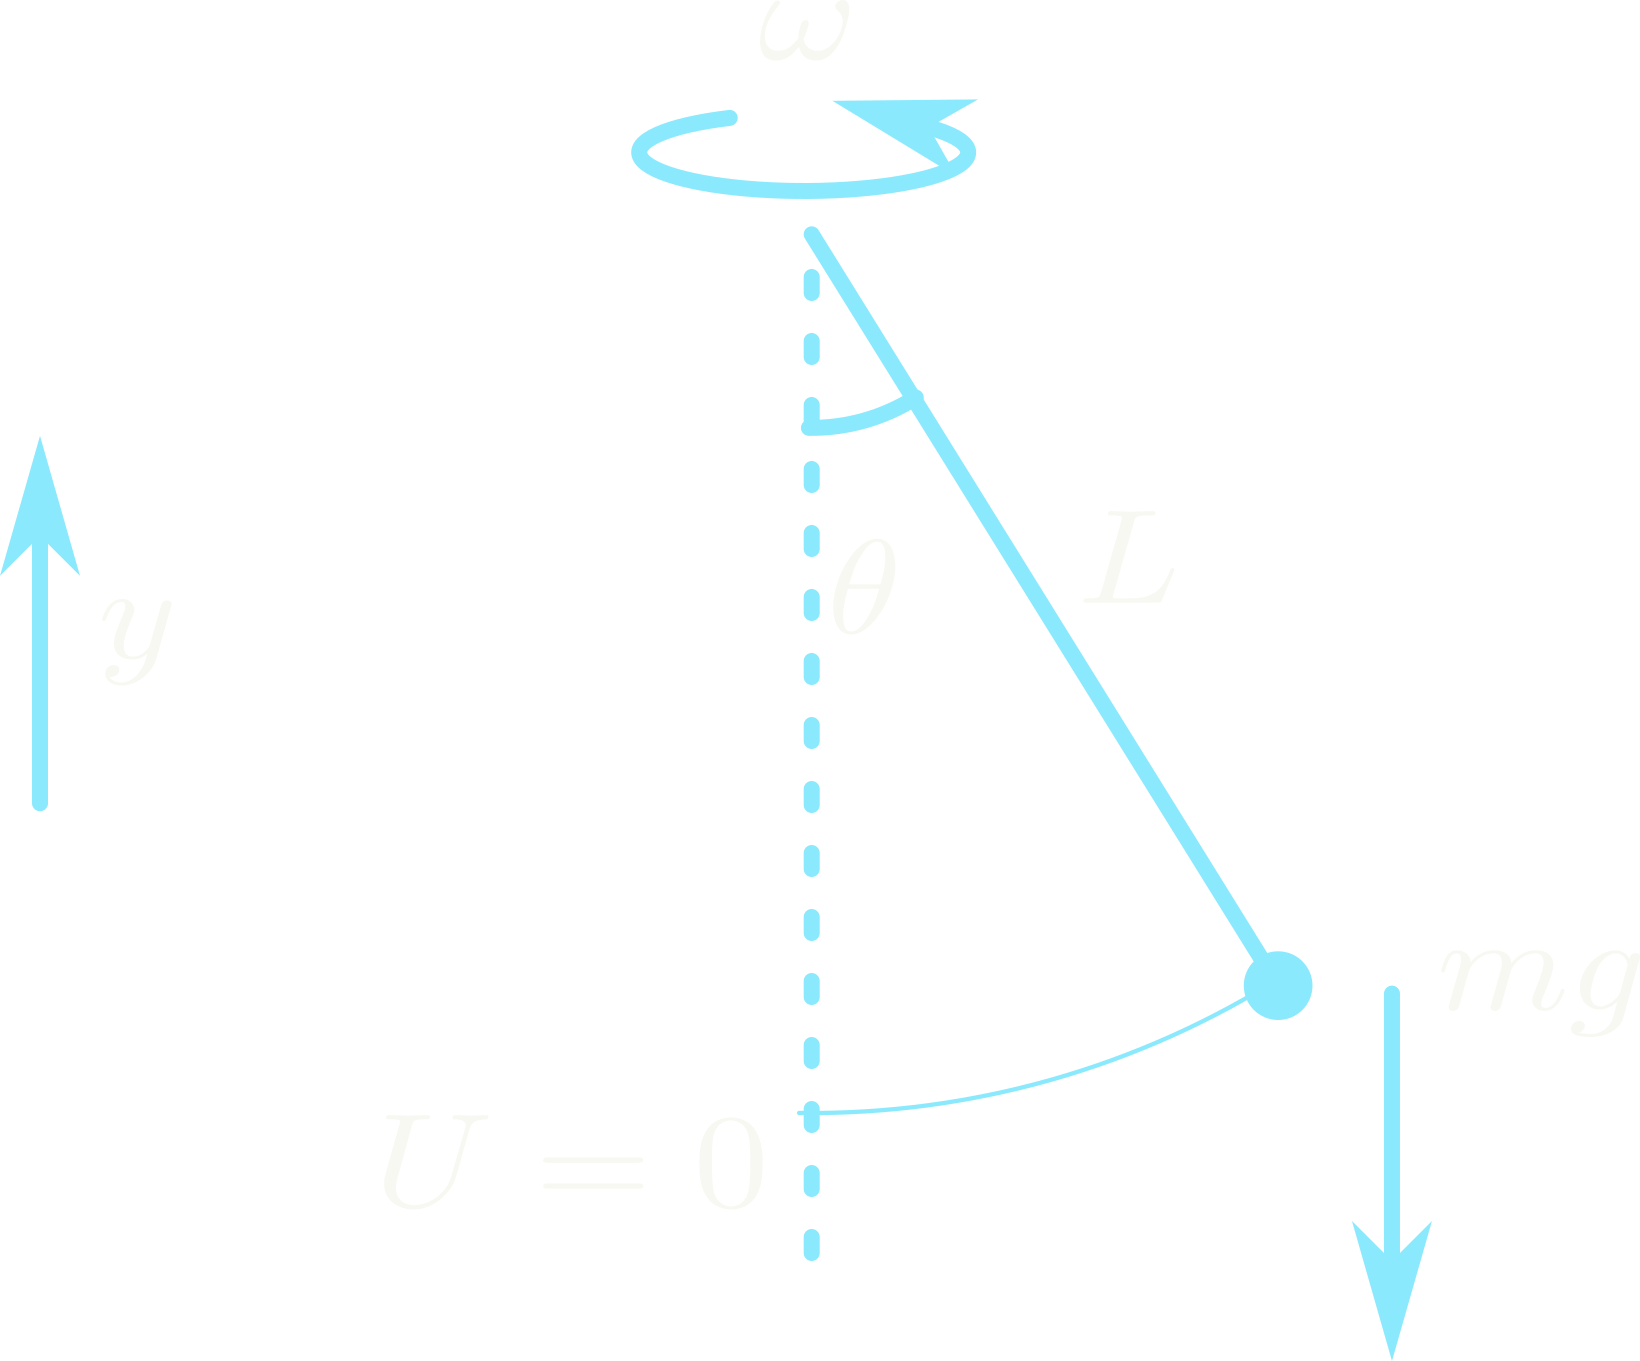
\includegraphics[width=0.5\textwidth]{spinningpendulum.png}
    \caption{Pendulum}
\end{figure}
\begin{align*}
    T &= \frac{1}{2} m v^2 = \frac{1}{2} m ((\omega L \sin \theta)^2 + (L \dot \theta)^2) \\
    U &= mg y = mg L (1 - \cos \theta)
\end{align*}
from EL equation we get
\begin{align*}
    \pdv{\lagr}{\theta} &= \frac{1}{2} m\omega^2 L^2 (2 \sin\theta \cos\theta) - mg L \sin\theta 
        = m\omega^2 L^2 \cos \theta \sin \theta - mgL \sin\theta \\
    \pdv{\lagr}{\dot \theta} &= m L^2 \dot \theta \\
    \dv{t} \pdv{\lagr}{\dot \theta} &= m L^2 \ddot \theta
\end{align*}
so 
\begin{align*}
    m L^2 \ddot \theta &= m\omega^2 L^2 \cos \theta \sin \theta - mgL \sin\theta \\
    \ddot \theta &= \omega^2 \cos \theta \sin \theta - \frac{g}{L} \sin \theta
\end{align*}
when $\omega = 0$ we get the simple pendulum $\ddot \theta = - \frac{g}{L} \sin \theta$. Identifying
the the equilibrium points where $\ddot \theta = 0 \implies$
\begin{align*}
    \sin \theta = 0 \implies \theta = 0, \pi
\end{align*}
at $\theta = 0$ the pendulum is just hanging vertically down which we can physically deduce as a
stable equilibrium point. To check this analytically we can assume a small deviation from the
equilibrium point:
\begin{align*}
    \theta &= 0 + \epsilon \\
    \cos(0 + \epsilon) &= 1 - \frac{\epsilon^2}{2} \approx 1 \\
    \sin(0 + \epsilon) &= \epsilon - \frac{\epsilon^3}{6} \approx \epsilon \\
\end{align*}
and we get
\begin{align*}
    \ddot \theta &= (\omega^2 - \frac{g}{L}) \theta \\
    \ddot \theta &= - \Omega^2 \theta \implies \mathrm{Stable} \\
    \ddot \theta &= \Omega^2 \theta \implies \mathrm{Unstable}
\end{align*}
where 
\begin{align*}
    \omega^2 < \frac{g}{L} \implies \mathrm{Stable} \\
    \omega^2 > \frac{g}{L} \implies \mathrm{Unstable}
\end{align*}
when they are equal $\omega^2 = \frac{g}{L}$ we get a simple pendulum. Finding another equilibrium
point at
\begin{align*}
    \omega^2 \cos\theta - \frac{g}{L} &= 0 \\
    \cos\theta &= \frac{g}{L\omega^2}, \qquad \theta = \pm \arccos(\frac{g}{L\omega^2})
\end{align*}
where there only exists a solution when
\begin{align*}
    \omega^2 > \frac{g}{L}
\end{align*}
since $\cos\theta \leq 1$. For this case, we can also look at the radial force in polar:
\begin{align*}
    F_r = m\ddot r - mr \omega^2
    \qor m\ddot r = F_r + mr \omega^2
\end{align*}
where in the second equation we can see that the sum of the centrifugal force and $F_r$ sums to zero
so
\begin{align*}
    \tan \theta = \frac{F_r}{mg} = \frac{mL \sin\theta\omega^2}{mg} \\
    \implies \frac{L\omega^2}{g} = \frac{1}{\cos\theta} \\
    \cos\theta = \frac{g}{L\omega^2}
\end{align*}
from the force analysis we can see that the centrifugal force is balanced by the radial force.
Substituing the equilibium position back into the EOM 
\begin{align*}
    \cos\theta_o = \frac{g}{L\omega^2} \to \theta = \theta_o + \epsilon
\end{align*}
Using Taylor Expansion, $f(x) = f(x_o) + f'(x_o) (x-x_o)$, the sine and cosine terms are
\begin{align*}
    \cos\theta &= \cos(\theta_o + \epsilon) = \cos\theta_o - \sin\theta_o \epsilon \\
    \sin\theta &= \sin(\theta_o + \epsilon) = \sin\theta_o + \cos\theta_o \epsilon
\end{align*}
so the EOM becomes
\begin{align*}
    \ddot \theta = (- \omega^2 \sin\theta_o \epsilon) (\sin\theta_o + \cos\theta_o \epsilon) \\
    \ddot \epsilon = -\omega^2 \sin^2(\theta_o) \epsilon
\end{align*}
where we have Bifurcation at $\omega^2 = \frac{g}{L}$. We can see that the EOM for $\epsilon$ is
similar to the harmonic oscillator so:
\begin{align*}
    \epsilon = A \cos(\Omega t - \delta) \qquad \Omega = \omega \sin\theta_o
\end{align*}
\paragraph*{HW 5} Given $f(x, y, y')$. Independence of $y$ means:
\begin{align*}
    f(x, y') \implies \pdv{f}{y'} = constant \\
    \lagr(t, \dot q) \implies \pdv{\lagr}{\dot q} = constant
\end{align*}
so for the Lagrangian
\begin{align*}
    \lagr &= T - U = \frac{1}{2} m \dot x^2 - U(x) \qquad \pdv{\lagr}{q_i} = F_i \qqtext{generalized force} \\
    \pdv{\lagr}{\dot x} &= m \dot x = conserved, \quad \pdv{U}{x} = 0
\end{align*}
if $\lagr$ doesn't depend on $x$, then $p_x$ (momentum) is conserved. So for the generalized 
Lagrangian
\begin{align*}
    \lagr(q_1, \dots, q_n, \dot q_1, \dots, \dot q_n, t) \\
    \mathrm{If} \quad \pdv{\lagr}{q_i} = 0, \quad  \pdv{\lagr}{\dot q_i} = \mathrm{conserved}
\end{align*}
So symmetry $\implies$ conservation (Noether's Theorem).

\newpage
\subsection*{Lecture 14: \hfill 2/21/24}
\hrule \vspace{10px}

\paragraph*{Conservation} The two types: 
\begin{itemize}
    \item If $f(x, y')$ is independent of $y$, then
    \begin{align*}
        \pdv{f}{y'} = \text{constant over } x
    \end{align*}
    or if $\lagr$ is independent of $q_i$, then
    \begin{align*}
        \pdv{\lagr}{q_i} = \text{constant over } t = p_i
    \end{align*}
    \item If $f(y, y')$ is independent of $x$, then
    \begin{align*}
        f - y' \pdv{f}{y'} = \text{constant over } x
    \end{align*}
    or if $\lagr$ is independent of $t$, then
    \begin{align*}
        \lagr - \dot q_i \pdv{\lagr}{\dot q_i} = \text{constant over } t
    \end{align*}
\end{itemize}
looking at this more closely:
    \begin{align*}
        \lagr &= T - U = \frac{1}{2} m \dot q^2 - U(q)
    \end{align*}
    where
    \begin{align*}
        \dot q \pdv{\lagr}{\dot q} &= m \dot q^2; \\
        \dot q \pdv{\lagr}{\dot q} - \lagr &= m \dot q^2 - \frac{1}{2} m \dot q^2 + U \\
        &= \frac{1}{2} m \dot q^2 + U = T + U = E
    \end{align*}
    this is this Hamiltonian 
    \begin{align*}
        \sum_i p_i \dot q_i - \lagr = \mathcal H = E
    \end{align*}
\paragraph*{Noether's Theorem} For a system independent of $t \leftrightarrow$ the system has
time-translation symmetry

$\implies$ conservation of energy

\paragraph*{Dependence on $t$} $U = U(q, t)$ e.g. Mass of sun is increasing over time, the potential
energy is dependent on time, so the system is not conservative. 

\paragraph*{Pendulum thoughts:} In our pendulum example, we chose $q = \theta$, but we could also
choose $q_1 = x$ and $q_2 = y$. The truth lies in the fact that we intuitively chose $q_1 = r$ and
$q_2 = \theta$. So in transforming from Cartesian coordinates
\begin{align*}
    x = r\cos\theta, \qquad y = r\sin\theta, \qquad r = L
\end{align*}
where we have a `constraint' $r = L$\dots

\paragraph*{Legal Terms: Formal Definition of Constraints} In the beginning, we defined the first defined position with
\begin{align*}
    \vb r = (x, y, z)
\end{align*}
for the generalized coordinates we have
\begin{align*}
    \vb r = \vb r(q_1, \dots, q_n, t)
\end{align*}
where we decided that in a 3D system $n = 3$. A constraint is an equation
\begin{align*}
    f(q_1, \dots, q_n) = 0
\end{align*}
where this is a \emph{holonomic} (whole) constraint and to find the number of generalized coordinates:
\begin{align*}
    \text{\# of generalized coordinates we need} &= \text{\# of dimensions} - \text{\# of constraints}  \\
    &= \text{\# of degrees of freedom}
\end{align*}
this is only true for holonomic constraints. For \emph{nonholonomic} constraints, it is more complicated
e.g. A ball on a horizontal table: We can see that \# of generalized coordinates = 2, but to
describe the position of the ball i.e. a dot on the ball, we need 3 more coordinates (Euler angles).
So the configuration of the ball is described by 5 coordinates $(x, y, \alpha, \beta, \gamma)$. In
other words, the configuration is path dependent and we see a nonholonomic constraint.

\paragraph*{Example:} What are the constraints for the mass sliding down a moving mass? The 
holonomic constraints are the vertical position of the ramp $y_M = 0$, and from $x_m, y_m, x_M$ we 
know the $x_{COM} =$ constant.

\paragraph*{Fact!} A constraint is enforced by a constraint force $\vb F_c \perp$ path(in the
pendulum example, the normal force $N$). Finding this force where $f(q_i) = 0$ can be found by
taking the gradient of the function $\grad f$. So
\begin{align*}
    \vb F_c = \lambda \grad f
\end{align*}

\newpage
\subsection*{Lecture 15: \hfill 2/23/24}
\hrule \vspace{10px}
\paragraph*{Review}
\begin{itemize}
    \item Convservation: Lagrangian is independent of time $\implies$ conservation of energy
\end{itemize}

\paragraph*{Lagrange Multiplier} Want to find $q_i(t)$ by minimizing
$S = \int \lagr(q_i, \dot q_i, t) \dd t$.
\paragraph*{} $\star$ Under holonomic constraints,
\begin{align*}
    f(q_i) = 0
\end{align*}
So we introduce a new unknown $\lambda(t)$ and the new minimizing integral becomes
\begin{align*}
    I = \int (\lagr - \lambda f) \dd t
\end{align*}
The EL eqn for $\lambda(t):\quad f=0$
\begin{align*}
    \pdv{(\lagr - \lambda f)}{\lambda} = -f \qquad \pdv{(\lagr - \lambda f)}{\dot \lambda} = 0
\end{align*}
The EL eqn for $q_i(t)$:
\begin{align*}
    F_i = \pdv{(\lagr - \lambda f)}{q_i} = \dv{t} \pdv{(\lagr - \lambda f)}{\dot q_i}
\end{align*}
or
\begin{align*}
    F_i = \pdv{\lagr}{q_i} - \lambda \pdv{f}{q_i} \qqtext{where} \pdv{\lagr}{q_i} = p_i
\end{align*}
So we are given $N+1$ unknowns and $N+1$ EL eqns with the addition of the lagrange multiplier.
\paragraph*{Simple Pendulum (revisited)} We have the Lagrangian
$\lagr(x, y, \dot x, \dot y) = T - U$ where 
\begin{align*}
    T &= \frac{1}{2} m (\dot x^2 + \dot y^2) \\
    U &= -mgy
\end{align*}
so
\begin{align*}
    \lagr = \frac{1}{2} m (\dot x^2 + \dot y^2) + mgy
\end{align*}
and using the constraint of the fixed length; $f(x, y) = x^2 + y^2 - L^2 = 0$ we get
\begin{align*}
    \ell = \lagr - \lambda f = \frac{1}{2} m (\dot x^2 + \dot y^2) + mgy - \lambda(x^2 + y^2 - L^2)
\end{align*}
and the EL eqns are
\begin{itemize}
    \item $x$:
    \begin{align*}
        -2\lambda x = m \ddot x
    \end{align*}
    \item $y$:
    \begin{align*}
        mg - 2\lambda y = m \ddot y
    \end{align*}
    \item $\lambda$: Left as an exercise
\end{itemize}
We can see from force analysis of the pendulum:
\begin{align*}
    m\ddot x = F_x = -2\lambda x \qquad m\ddot y = F_y = mg - 2\lambda y
\end{align*}
so the lagrange multiplier quantities are equivalent to the tension
\begin{align*}
    T_x = 2\lambda x \qquad T_y = 2\lambda y
\end{align*}
where the negative sign indicates the correct direction of Tension.

\paragraph*{Pendulum in Polar} $(r, \phi)$
\begin{align*}
    \lagr(r, \phi, \dot r, \dot \phi) = \frac{1}{2} m (\dot r^2 + r^2 \dot \phi^2) - mgr\cos\theta
\end{align*}
where
\begin{align*}
    f = r - L = 0
\end{align*}
so we get the EL eqns
\begin{align*}
    -\lambda + mg\cos\theta = m\ddot r \qquad \lambda = mg\cos\theta
\end{align*}

\paragraph*{Use cases of Lagrange Multipliers} Although the previous example seems trivial, we 
consider its use in the example of a heavy chain hanging from two poles: The linear mass density is
given by
\begin{align*}
    M = \rho L
\end{align*}
to find the shape, we need to minimize the potential energy
\begin{align*}
    S = \int \dd m g y
\end{align*}
where $\dd m = \rho \dd s$ is the mass of a segment and under the constraint of chain length:
\begin{align*}
    L = \int \dd s = \int \dd x \sqrt{1 + y'^2} 
\end{align*}
so
\begin{align*}
    S = \int \rho gy \sqrt{1 + y'^2} \dd x
\end{align*}
and introducing $\lambda$ we minimize
\begin{align*}
    \int (\rho g y - \lambda) \sqrt{1 + y'^2} \dd x = S - \lambda L
\end{align*}
we can see that it is independent of $x$ so
\begin{align*}
    f = (\rho g y - \lambda) \sqrt{1 + y'^2}
\end{align*}
and
\begin{align*}
    f - y' \pdv{f}{y'} = \text{constant} = C
\end{align*}
so the EL eqn is:
\begin{align*}
    \pdv{f}{y'} = (\rho g y - \lambda) \frac{y'}{\sqrt{1 + y'^2}}
\end{align*}
and therefore
\begin{align*}
    f - y' \pdv{f}{y'} = (\rho g y - \lambda)
        \qt[\sqrt{1 + y'^2} - \frac{y'^2}{\sqrt{1 + y'^2}}] = \text{constant}
\end{align*}
and quantity in brackets is
\begin{align*}
    [\;] = \frac{1}{\sqrt{1 + y'^2}}
\end{align*}
so
\begin{align*}
    \qt(\frac{\rho g y - \lambda}{\sqrt{1 + y'^2}})^2 &= C^2 \\
    1 + y'^2 &= \frac{(\rho g y - \lambda)^2}{C^2}
\end{align*}
for an easier solution we choose a change of variables
\begin{align*}
    \tilde y = \frac{\rho g y - \lambda}{C} \implies \tilde y' = \frac{\rho g}{C} y'
\end{align*}
and redifining the $x$
\begin{align*}
    \tilde y'^2 = 1 + y'^2
    \begin{cases}
        \tilde x = \frac{\rho g}{C} x \\
        \dv{\tilde y}{\tilde x} = \dv{y}{x}
    \end{cases}
\end{align*}
and we get
\begin{align*}
    \tilde y = \pm \cosh(\tilde x - \tilde x_0)
\end{align*}
we could have also used the Lagrange Multiplier for the Maximum Area Fixed Perimeter problem.

\newpage
\subsection*{Lecture 16: \hfill 2/26/24}
\hrule \vspace{10px}

\paragraph*{Review} Constraint -- holonomic $\quad f(q,\dots, q_n) = 0 \to$ Lagrange Multiplier
\paragraph*{Example} Simple pendulum spinning on its vertical axis. We have the Lagrangian
\begin{align*}
    T &= \frac{1}{2} m(L^2 \dot\theta^2 + L^2 \sin^2\theta \omega^2) \\
    U &= mgy = mgL(1 - \cos\theta) \\
    \lagr &= T - U \\
    &= \frac{1}{2} m L^2 \dot \theta^2 + \frac{1}{2} m L^2 \sin^2\theta \omega^2 + mgL(1 - \cos\theta)
\end{align*}
but we can see the derivatives are also conserved:
\begin{align*}
    T' &= \frac{1}{2} m L^2\dot\theta^2, \quad U' = -\frac{1}{2} mL^2 \omega^2 \sin^2\theta + mg(1 - \cos\theta) \\
    \lagr &= T' - U'
\end{align*}
where $U'$ is called the effective potential. $E'$ is conserved, so
\begin{align*}
    \pdv{\lagr}{\dot\theta} &= ml^2 \dot\theta \qqtext{angular momentum} \\
    \dot\theta\pdv{\lagr}{\dot\theta} - \lagr &= E' \\
    &= \frac{1}{2} mL^2 \dot\theta^2 - \frac{1}{2} mL^2\omega^2 \sin^2\theta + mgL(1 - \cos\theta) = T' + U' \\
    T + U &= \frac{1}{2}mL^2\dot\theta^2 + \frac{1}{2} mL^2\omega^2 \sin^2\theta + mgL(1 - \cos\theta)
\end{align*}
we can see that the conserved quantity is different the mechanical energy $E = T + U$. We should be
careful with finding what is the conserved quantity in noninertial frames (mechanical energy is not
always conserved). In order to study the the function, we should look at the $E'$ term.
\paragraph*{} Equilibrium points:
\begin{align*}
    \dv{U'}{\theta} = 0 \\
    (g - L \omega^2 \cos\theta) \sin\theta = 0
\end{align*}
\begin{itemize}
    \item if $\omega^2 < \frac{g}{L}$ then only 1 equilibrium point 
    \item if $\omega^2 > \frac{g}{L}$ then 2 equilibrium points
\end{itemize}
\begin{figure}[ht]
    \centering
    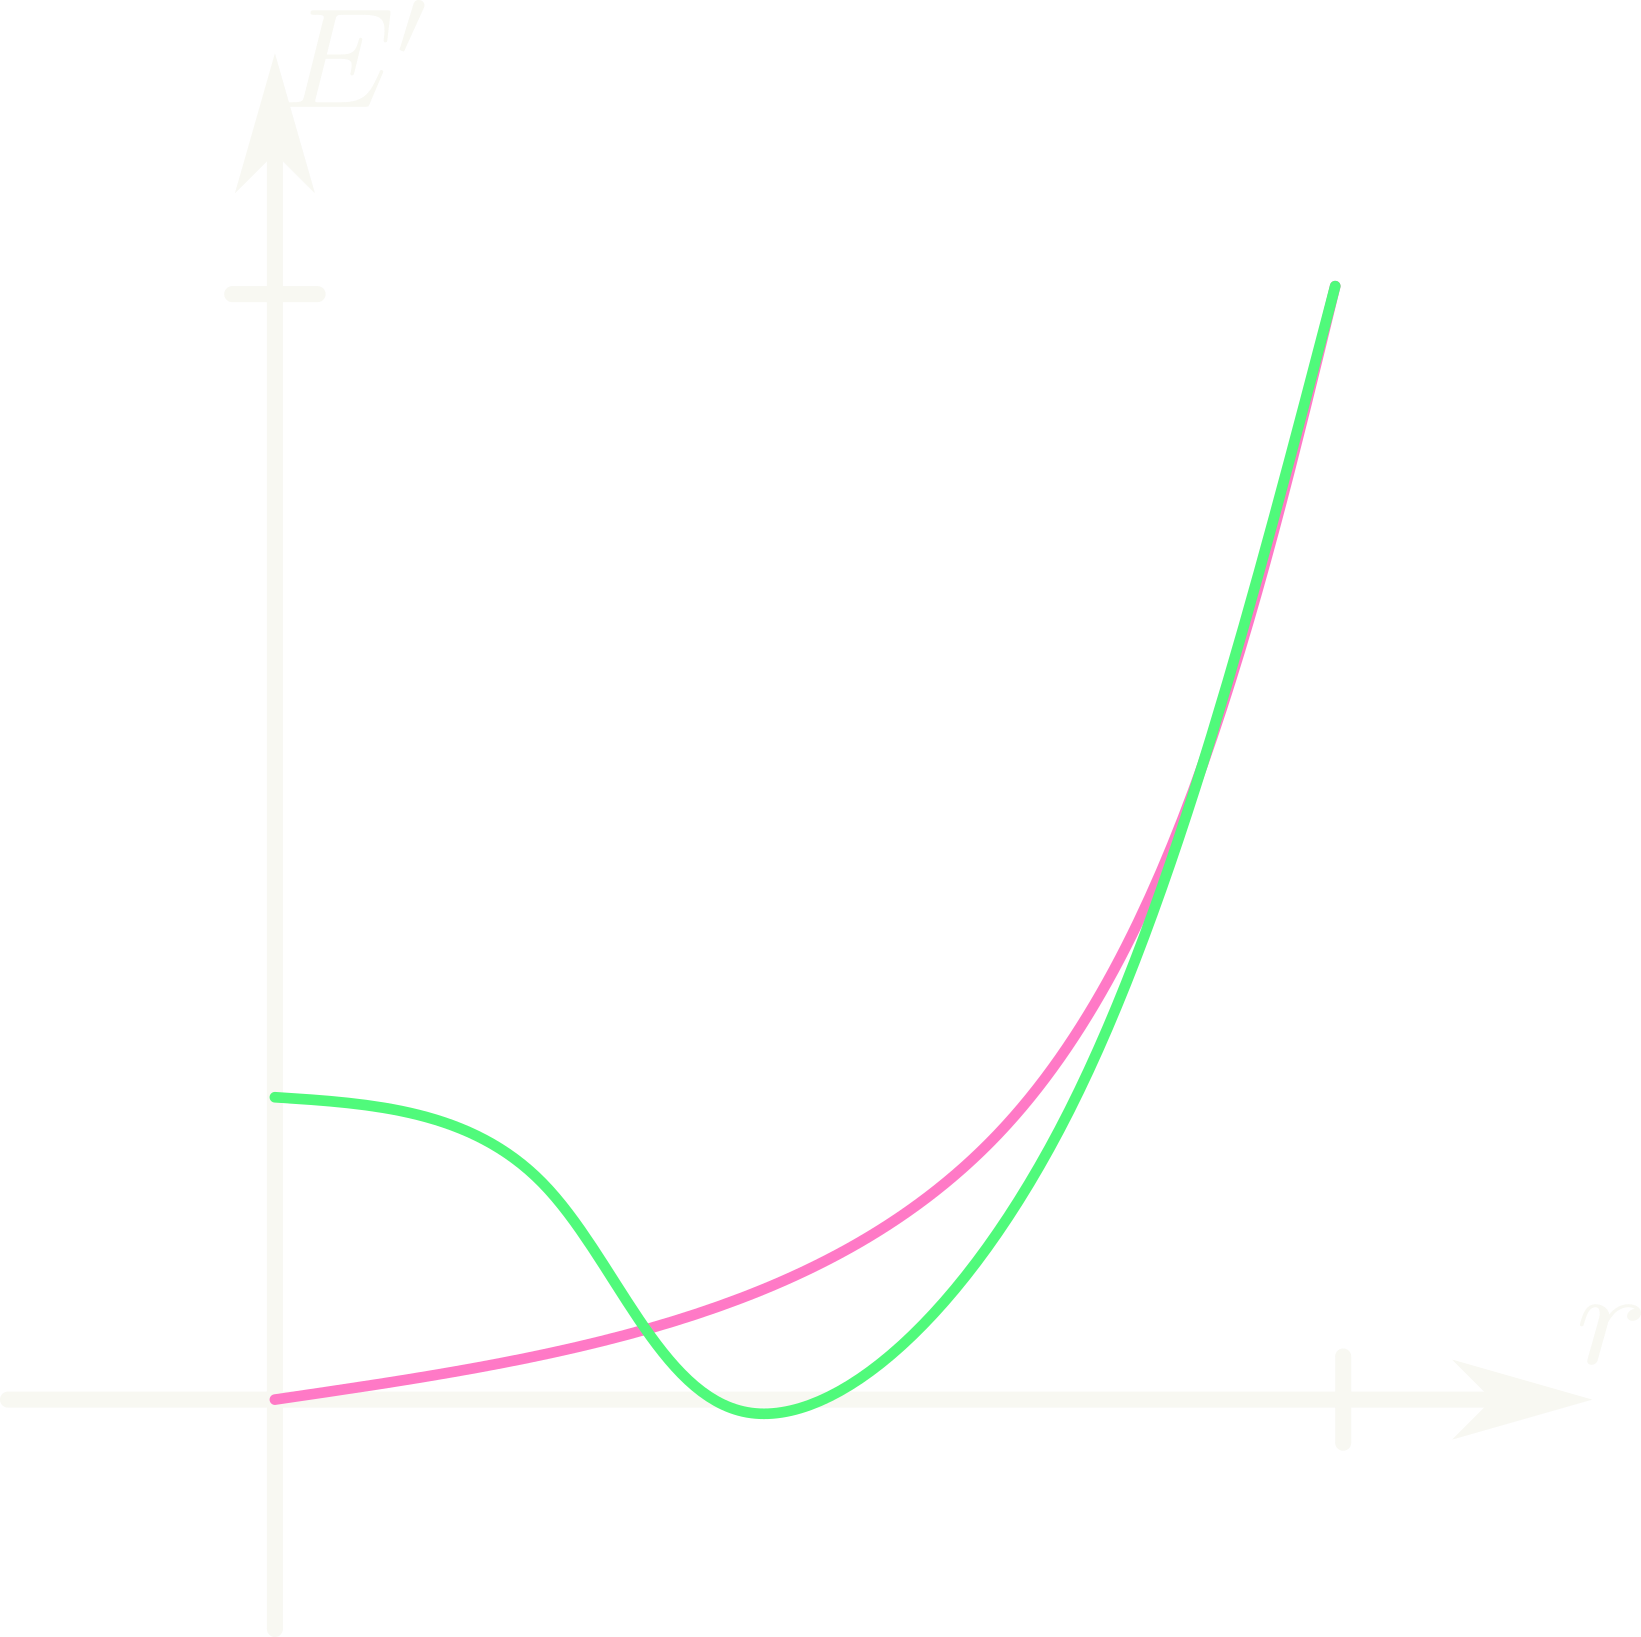
\includegraphics[width=0.4\textwidth]{mexicanhat.png}
    \caption{Red shows 1 eq point, green shows 2 eq points}
    \label{fig:mexicanhat}
\end{figure}
Figure \ref{fig:mexicanhat} shows the effective potential $U'(\theta)$ for the two cases. Sidenote:
spinning the green curve around the $E'$ axis gives rise to the Mexican Hat potential in particle
physics(Higgs Boson!). 

\paragraph*{Lagrangian for a charged particle} $\vb E, \vb B$: we have a Lorentz force
\begin{align*}
    m\vb a = F  = q(\vb E + \vb v \times \vb B)
\end{align*}
where we can define a vector potential $\vb A$ such that
\begin{align*}
    \vb E = -\grad \phi - \pdv{\vb A}{t}, \quad \vb B = \curl \vb A
\end{align*}
Goal: to find $\lagr$ that gives
\begin{align*}
    \pdv{\lagr}{q} &= \dv{t}(\pdv{\lagr}{\dot q})
\end{align*}
so
\begin{align*}
    \lagr = \frac{1}{2} m \vb v^2 - q(\phi - \vb v \cdot \vb A)
\end{align*}
the generalized coordinate is $q(x, y, z)$ and we just look at $x$:
\begin{align*}
    \pdv{\lagr}{x} &= -q\dv{\phi}{x} + q \vb v \cdot \pdv{\vb A}{x} \\
       &= -q\qt(\dv{\phi}{x} + v_x \pdv{A_x}{x} + v_y \pdv{A_y}{x} + v_z \pdv{A_z}{x})  \\
    \pdv{\lagr}{\dot x} &= m v_x + q A_x
\end{align*}
so from the total derivative
\begin{align*}
    \dv{t} = \pdv{t} + \dv{x}{t} \pdv{x} + \dv{y}{t} \pdv{y} + \dv{z}{t} \pdv{z}
\end{align*}
we get
\begin{align*}
    \dv{t}(\pdv{\lagr}{\dot x}) &= m \dot v_x + q(\cancel{v_x \pdv{A_x}{x}} + v_y \pdv{A_x}{y} + v_z \pdv{A_x}{z} + \pdv{A_x}{t}) \\
\end{align*}
so 
\begin{align*}
    m \dot v_x = ma_x &= -q\qt(\pdv{\phi}{x} - \pdv{A_x}{t}) \qquad \equiv qE_x \\
    &\quad + qv_y \qt(\pdv{A_y}{x} - \pdv{A_x}{y}) \qquad \equiv B_z \\
    &\quad - qv_z \qt(\pdv{A_x}{z} - \pdv{A_z}{x}) \qquad \equiv B_y \\
    &= qE_x + qv_y B_z - qv_z B_y
\end{align*}
which is the Lorentz force. We can think of the momentum as
\begin{align*}
    \pdv{\lagr}{\dot q_i} = p_i \qquad \vb p = m \vb v + q \vb A
\end{align*}
and from QM we know
\begin{align*}
    \vb p \to -i\hbar \grad - q \vb A
\end{align*}
And reviewing from Chapter 2, the linear drag force
\begin{align*}
    \vb f = -b \vb v
\end{align*}
is obviously nonconservative. So can get the EL eqn quickly by adding this force to the generalized
force
\begin{align*}
    \dv{t}(\pdv{\lagr}{\dot q_i}) &= \pdv{\lagr}{q_i} + f \\
    p_i = F + f
\end{align*}
this comes from Rayliegh dissipation function.
\begin{align*}
    R(\dot q) = \frac{1}{2} b \dot q^2 \qquad f = - \pdv{R}{\dot q}
\end{align*}
so the EL eqn is
\begin{align*}
    \dv{t}(\pdv{\lagr}{\dot q}) - \pdv{\lagr}{q} = - \pdv{R}{\dot q}
\end{align*}
where we have functions 
\begin{align*}
    T(\dot q), U(q), R(\dot q)
\end{align*}
so
\begin{align*}
    \dv{t}(\pdv{T}{\dot q}) + \pdv{R}{\dot q} + \pdv{U}{q} = 0
\end{align*}

\newpage
\subsection*{Lecture 17: \hfill 2/28/24}
\hrule \vspace{10px}

\paragraph{Midterm Review} 
\begin{itemize}
    \item Newton's Laws
    \begin{itemize}
        \item 1. Inertial: Keep on going and it won't stop coming, so much to do so much to see. 
        \item 2. $\vb F =m \vb a = m \ddot{\vb r}$
        \item 3. $\vb F_{12} = -\vb F_{21}$
    \end{itemize}
    \item Polar Coordinates $(r, \phi)$
    \begin{align*}
        \begin{cases}
            x = r\cos\phi \\
            y = r\sin\phi
        \end{cases}
    \end{align*}
    and unit vectors are orthogonal
    \begin{align*}
        \begin{cases}
            \hat r = \cos\phi \hat x + \sin\phi \hat y \\
            \hat \phi = -\sin\phi \hat x + \cos\phi \hat y
        \end{cases}
        \to \vu r \cdot \vu*\phi = 0
    \end{align*}
    such that the unit vector time derivatives are
    \begin{align*}
        \dot{\vu r} = \dot \phi \vu*\phi \\
        \dot{\vu*\phi} = -\dot\phi \vu r
    \end{align*}
    so the velocity and acceleration is actually
    \begin{align*}
        \vb v = \dot{\vb r} &= \dot r \vu r + r \dot\phi \vu*\phi \\
        &= v_r \vu r + v_\phi \vu*\phi \\
        \vb a &= (\ddot r - r \dot\phi^2) \vu r + (2\dot r \dot\phi + r \ddot\phi) \vu*\phi \\
        &= a_r \vu r + a_\phi \vu*\phi
    \end{align*}
    where the forces are
    \begin{align*}
        F_r = ma_r \qquad F_\phi = ma_\phi
    \end{align*}
    \item Momentum $\vb p = m \vb v$ and in relation to force $\vb F = \dv{\vb p}{t}$. For a
    collection of particles, the total external force is
    \begin{align*}
        \dv{t} \sum_i \vb p_i = \vb F_{ext}
    \end{align*}
    \item Angular momentum
    \begin{align*}
        \vb \ell = \vb r \times \vb p
    \end{align*}
    \item Center of mass
    \begin{align*}
        \vb R &= \frac{1}{M} \sum m_i \vb r_i \qquad M = \sum m_i \\
        \vb R &= \frac{1}{M} \int \vb r \dd m
    \end{align*}
    \item Energy: Kinetic energy is
    \begin{align*}
        T = \frac{1}{2} mv^2 = \frac{1}{2} m \vb v \cdot \vb v
    \end{align*}
    and for the two coordinate systems:
    \begin{align*}
        v^2 = v_x^2 + v_y^2 = v_r^2 + v_\phi^2
    \end{align*}
    \item Work-KE Theorem: 
    \begin{align*}
        T_2 - T_1 = \int_1^2 \vb F \cdot \dd \vb r = W(1 \to 2)
    \end{align*}
    and if $\vb F$ is conservative---only depends on position: $\vb F(\vb r)$ \& $\curl \vb F = 0$
    thus $\vb F = -\grad U$---then
    \begin{align*}
        W(1 \to 2) = -\Delta U = U_1 - U_2 \\
        E = T_1 + U_1 = T_2 + U_2
    \end{align*} 
    and more closely finding the critical points of $U$ i.e.
    \begin{align*}
        \pdv{U}{x} = 0 \qor \grad{U} = 0
    \end{align*}
    we also have classical turning points when $E = U$. (Not too important) For the case
    \begin{align*}
        \frac{1}{2} m \dot x^2 = E - U(x) \\
        \implies \dot x = \dv{x}{t} = \sqrt{\frac{2}{m}} \sqrt{E - U(x)}
    \end{align*}
    \item Oscillators
    \begin{align*}
        \ddot x = -\frac{k}{m} x = -\omega_o^2 x \qquad \omega_o = \sqrt{\frac{k}{m}}
    \end{align*}
    the solution is written in several forms:
    \begin{align*}
        x(t) &= B_1 \cos(\omega_o t) + B_2 \sin(\omega_o t) \\
        &= \Re [C_1 e^{i\omega_o t} + C_2 e^{-i\omega_o t}] \\
        &= A \cos(\omega_o t - \delta)
    \end{align*}
    where we solve for the constants using the initial conditions $x(0) = x_o, \quad \dot x(0) = v_o$
    \item Damped Oscillators:
    \begin{align*}
        \ddot x + 2\beta \dot x + \omega_o^2 x = 0
    \end{align*}
    where we have a homogeneous solution for the three cases:
    \begin{itemize}
        \item $\beta = \omega_o$: Critical damping
        \begin{align*}
            x_h(t) = e^{-\beta t}(C_1 + C_2 t)
        \end{align*}
        \item $\beta > \omega_o$: Overdamping
        \begin{align*}
            x_h(t) = e^{-(\beta - \sqrt{\beta^2 - \omega_o^2})t}
                \qt( C_1 + C_2 e^{-2\sqrt{\beta^2 - \omega_o^2}t})
        \end{align*}
        \item $\beta < \omega_o$: Underdamping (weak damping)
        \begin{align*}
            x_h(t) = e^{-\beta t} A \cos(\omega t - \delta) \qquad \omega = \sqrt{\omega_o^2 - \beta^2}
        \end{align*}
    \end{itemize}
    \item Driven Damped Oscillators:
    \begin{align*}
        \ddot x + 2\beta \dot x + \omega_o^2 x = f_0 \cos(\omega t)
    \end{align*}
    where $f_o$ has units of acceleration and $\beta$ has units of frequency. The solution is always
    \begin{align*}
        x(t) = A \cos(\omega t - \delta) + x_h(t)
    \end{align*}
    where $x_h(t)$ is the transient solution and the constants are
    \begin{align*}
        A^2 = \frac{f_0^2}{(\omega_o^2 - \omega^2)^2 + 4\beta^2 \omega^2} \qquad 
        \delta = \arctan(\frac{2\beta \omega}{\omega_o^2 - \omega^2})
    \end{align*}
    where we have a resonance frequency around $\omega = \omega_o$.
    \item Calculus of Variations: minimizing the action
    \begin{align*}
        S = \int f(x, y, y') \dd x
    \end{align*}
    to find $y(x)$ from the EL eqn
    \begin{align*}
        \pdv{f}{y} = \dv{x}(\pdv{f}{y'})
    \end{align*}
    \item Lagrangian (Application of CoV)
    \begin{align*}
        \lagr = T - U
    \end{align*}
    where the EL eqns are
    \begin{align*}
        \pdv{\lagr}{q_i} = \dv{t}(\pdv{\lagr}{\dot q_i})
    \end{align*}
    \item Conservation: Two special cases
    \begin{itemize}
        \item If $\lagr$ is independent of $q_i \Leftrightarrow \pdv{\lagr}{q_i} = 0$
        \begin{align*}
            p_i \equiv \pdv{\lagr}{\dot q_i} = \text{is conserved}
        \end{align*}
        \item If $\lagr$ is independent of $t$
        \begin{align*}
            \mathcal H = \sum_i \dot q_i p_i - \lagr = \text{constant}
        \end{align*}
    \end{itemize}
\end{itemize}
\end{document}